\documentclass[conference,10pt]{IEEEtran}
\usepackage[T1]{fontenc}
\usepackage[utf8]{inputenc}
\usepackage{graphicx}
\usepackage{url}
\usepackage{array}
\usepackage{booktabs}
\usepackage{tabularx}
\usepackage{float}
\usepackage{placeins}
\usepackage[font=normalsize,labelfont=bf]{caption}
\captionsetup{skip=3pt}
\setlength{\textfloatsep}{5pt}
\setlength{\floatsep}{5pt}
\setlength{\intextsep}{5pt}
\begin{document}
\title{Group 4: Extending GenD for Video-Level Deepfake Detection Through Temporal GRUs and Score-Level Ensembles}
\author{\IEEEauthorblockN{Aashish Dahal, Suyog Acharya, Sanskar Bajimaya, Amir Karki}\IEEEauthorblockA{Fairleigh Dickinson University, Vancouver Campus}}
\maketitle
\begin{abstract}
Deepfake video detectors often lose accuracy when manipulation techniques and evaluation datasets change. GenD uses pretrained visual encoders to classify individual face crops, then averages frame probabilities to obtain a video score. This project examines whether chronological information and complementary image representations improve that approach without retraining the original visual encoders.

We trained separate gated recurrent units (GRUs) on CLIP and Perception Encoder (PE) features from 1,020 FaceForensics++ videos and compared six video-scoring configurations. On the 518-video Celeb-DF v2 external test set, the released GenD CLIP+PE score ensemble achieved 0.9712 AUROC, exceeding the combined GRU ensemble at 0.9640. The results distinguish strong in-domain temporal classification from cross-dataset generalization.

\end{abstract}
\clearpage
\section{INTRODUCTION}
Manipulated facial video can preserve a convincing identity and scene while introducing only limited visual evidence of synthesis. A detector must therefore distinguish subtle artifacts without relying on a particular generator, compression profile, or video source. GenD was developed to improve transfer between deepfake benchmarks through large pretrained visual encoders and targeted parameter adaptation \cite{yermakov2026}. The FaceForensics++ benchmark \cite{rossler2019} and the more challenging Celeb-DF v2 benchmark \cite{li2020} provide different evaluation settings for this problem.

A frame classifier is useful because facial manipulation frequently leaves local image evidence. However, GenD’s standard video inference reduces independent frame probabilities to one average \cite{yermakov2026}. This rule is invariant to frame order and cannot explicitly represent how visual features change over time. In addition, a single pretrained encoder may respond differently to manipulation artifacts from another encoder. Neither observation guarantees that a more complex classifier will generalize better, so both hypotheses require controlled experiments.

Our first research question is whether an ordered sequence of frozen GenD feature vectors supports better video-level classification than independent-frame probability averaging. We trained 32-frame and 64-frame CLIP-based GRUs and a 32-frame PE-based GRU. Each predicts one video label from a temporal hidden state. CLIP supplies transferable features \cite{radford2021}, RetinaFace aligns the input faces \cite{deng2020}, and GRU gates model ordered observations \cite{cho2014}. The second question is whether averaging scores from the released GenD-CLIP and GenD-PE heads, or from separately trained GRUs, reduces errors without mixing their underlying embeddings.

The study deliberately separates in-domain evidence from external validation. We partitioned 1,020 FaceForensics++ c23 videos by 255 related-source groups, so source-related originals and manipulations cannot cross training, validation, and test sets. Model selection used validation data before evaluation on 100 held-out FaceForensics++ videos. An additional 518 official Celeb-DF v2 test videos were evaluated without GRU retraining or threshold selection on that dataset. The public source repository preserves the evaluation outputs and documents a local Gradio demonstration \cite{capstone2026}.

The data provide a meaningful caution about model complexity. Averaged CLIP-GRU seed predictions yield a perfect ranking on the small in-domain test set, but the CLIP-GRU and PE-GRU perform less well on Celeb-DF v2 than the released-head ensemble. The outcome supports evaluating both ranking quality and low-false-positive operating points rather than choosing the largest in-domain score.

There are two distinct meanings of improved performance in this setting. An in-domain experiment asks whether a new classifier reduces mistakes on videos collected and manipulated under the conditions that supplied its training labels. A generalization experiment instead asks whether that improvement survives a change in the data-generating process. Both questions are valuable, but they require different evidence. A model may learn genuine video-level temporal structure and still attach too much weight to features that are common only to one manipulation process. For this reason, we report the experiments separately rather than combining their scores into a single success claim \cite{yermakov2026}, \cite{rossler2019}, \cite{li2020}.

The project also studies the cost of extra modeling. Standard GenD computes frame representations and applies a linear classification head. A GRU adds a learned recurrent stage and requires a fixed-order feature tensor, while a two-backbone ensemble needs two visual forward passes. The added work is justified only if it improves the operating characteristics that matter for screening videos. Our experiments therefore compare model rankings over all thresholds and recall under strict false-positive constraints. They also distinguish the mean of independent training-seed measurements from the result obtained after averaging saved seed probabilities for each video \cite{capstone2026}.

Reproducibility influenced the design from the beginning. All four source-related videos stay inside the same split; the largest full experiment uses five training seeds for each temporal setting; validation results determine the chosen configuration; and final benchmark scores come from saved video predictions. The project repository supplies model and preprocessing code, selected-configuration metadata, training logs, and cross-dataset output tables. These artifacts permit the quantitative claims in the report to be traced to a defined protocol without distributing restricted FaceForensics++ raw videos \cite{rossler2019}, \cite{capstone2026}.

The principal contributions of Group 4 are:

\begin{itemize}
\item A leakage-controlled temporal extension of GenD using frozen 1,024-dimensional CLIP and PE features, shared chronological frame positions, and five independently trained GRUs per configuration.
\item A reproducible comparison of released heads, temporal classifiers, and probability-level ensembles on a common FaceForensics++ test split and the external Celeb-DF v2 benchmark.
\item An analysis of cross-dataset limitations, paired bootstrap differences, and practical inference trade-offs, supported by saved results and a local demonstration.
\end{itemize}
\FloatBarrier
\clearpage
\section{BACKGROUND}
\subsection{Facial preprocessing and pretrained representations}
The detection pipeline begins with a decoded video, uniformly selected frame positions, and a face extraction stage. RetinaFace locates facial landmarks and identifies the largest usable face \cite{deng2020}. Each selected face is aligned, its bounding region is expanded by a factor of 1.3, and the image is resized to 224 × 224 pixels. Fig. 1 shows the shared frame-to-score architecture. This consistent policy is important because a detector should not obtain an artificial advantage from unequal preprocessing of the frame-averaging baseline and temporal models \cite{capstone2026}.

\begin{figure}[!htbp]
\centering
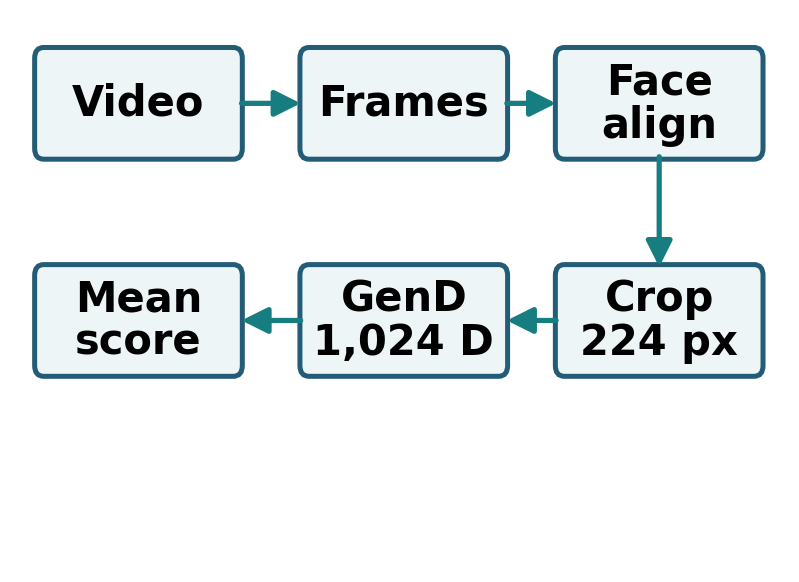
\includegraphics[width=0.98\columnwidth]{figures/fig01_gend_architecture.png}
\caption{Shared GenD frame-inference architecture, reconstructed from the team’s presentation. Arrows indicate data movement; the final video score averages frame-level probabilities.}
\label{fig:1}
\end{figure}
GenD builds on pretrained vision representations rather than learning all visual features from scratch \cite{yermakov2026}. CLIP’s transferable image features originate from large-scale image-text training \cite{radford2021}. In the released GenD configurations, a 1,024-dimensional classification-token feature is normalized and passed to a linear real/fake head. The original research emphasizes efficient adaptation of normalization parameters; our temporal experiments leave the released visual encoders unchanged \cite{yermakov2026}, \cite{capstone2026}.

The two released GenD backbones contribute complementary image representations, but they are not interchangeable model heads. Both accept aligned face images and expose visual features of the same reported dimensionality; a PE feature is computed by PE, not obtained by relabeling or converting a CLIP feature. That distinction matters in the temporal experiments: the matching frame IDs control which moment of a video is seen, while the encoder remains a deliberate experimental variable. It also makes probability-level fusion easier to interpret than raw feature concatenation. A common video score is required before their predictions can be compared \cite{yermakov2026}, \cite{capstone2026}.

\subsection{Temporal learning and video-level decisions}
For standard inference, GenD scores selected face crops separately and averages their fake-class softmax probabilities. Reordering those frames leaves the average unchanged. A gated recurrent unit instead maintains a hidden state while reading successive feature vectors. Reset and update gates regulate what information is retained from earlier inputs \cite{cho2014}. In our implementation a single-layer GRU maps the ordered 1,024-dimensional sequence to a 128-dimensional terminal hidden state; a linear head and sigmoid produce one video-level fake score \cite{capstone2026}. The GRU depends on the upstream encoder and cannot analyze raw video independently. Fig. 2 illustrates the separate encoder-to-GRU branches.

\begin{figure}[!htbp]
\centering
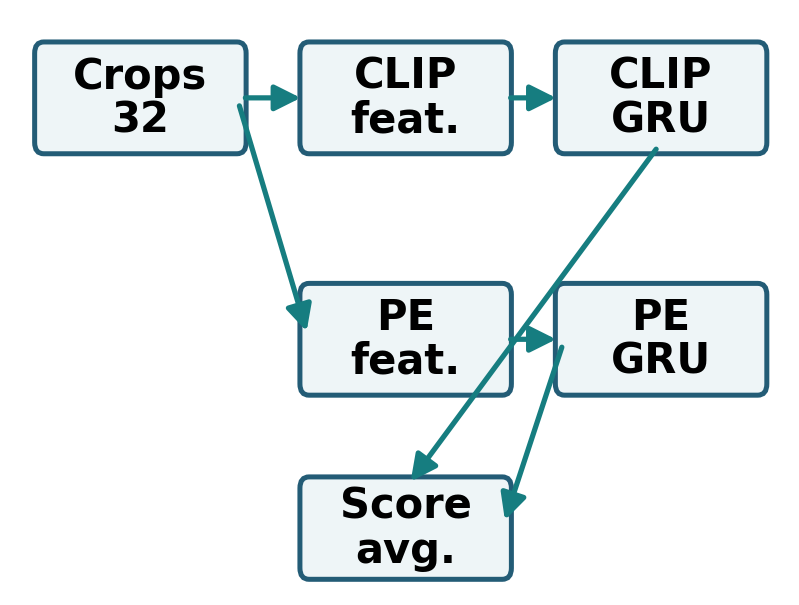
\includegraphics[width=0.98\columnwidth]{figures/fig02_temporal_architecture.png}
\caption{System architecture of the separate CLIP-GRU and PE-GRU branches. Two frozen encoders feed independent temporal classifiers; only final video scores are averaged.}
\label{fig:2}
\end{figure}
The 32-frame and 64-frame designs address a separate question about temporal sampling density. Using 64 ordered face crops offers more input observations but increases feature-extraction and sequence-processing requirements. A cached 64-frame master artifact can supply the 32-frame branch at alternating positions, avoiding an uncontrolled difference caused by independent frame sampling. The feature sequence must preserve chronological order, since a GRU hidden state depends on the positions at which observations are read. In contrast, the average of a set of frame scores stays unchanged if their order is shuffled \cite{capstone2026}.

\subsection{Fusion principles and evaluation metrics}
Score-level ensembling retains the different feature spaces and classification heads of the two backbones. Mean-probability fusion averages their fake scores; the team also examined mean-logit and mean-rank alternatives during the earlier ensemble study. Mean-rank fusion is an ordering statistic rather than a calibrated probability \cite{capstone2026}. The expanded final experiment uses common video-level mean-probability outputs to compare the released heads, each GRU seed ensemble, and their combinations.

The study also distinguishes validation decisions from test evaluation. Validation scores can choose the number of frames and the saved checkpoint for each seed; they do not estimate performance on new manipulation methods by themselves. Source-group-aware splitting prevents a reciprocal manipulated video from entering a different partition than its original. This precaution reduces an identifiable leakage route, but does not eliminate shared generator or compression characteristics across the dataset. The external benchmark remains necessary to evaluate that distribution shift \cite{rossler2019}, \cite{li2020}, \cite{capstone2026}.

Area under the receiver operating characteristic curve (AUROC) measures the ranking of genuine and manipulated videos across thresholds. Average precision (AP) summarizes the precision-recall trade-off; equal-error rate (EER) is the operating point where false-positive and false-negative rates coincide. Recall at 1\% false-positive rate is particularly relevant to screening systems because high overall AUROC may coexist with many false alarms. Test accuracy at a fixed 0.5 threshold should not be treated as a calibrated deployment estimate \cite{capstone2026}.

\subsection{Dataset grouping and experimental comparability}
FaceForensics++ includes related real and fake videos, which creates a potential shortcut if individual files are independently randomized into training and testing. A model could then encounter visually related faces, source identities, or recording conditions during training. Grouping the associated two originals and two reciprocal manipulations into one four-video unit reduces this risk. The resulting 204 training, 26 validation, and 25 test groups determine which examples may influence model parameters, which examples may guide selection, and which remain reserved for final measurement \cite{rossler2019}, \cite{capstone2026}.

This protocol controls one important source of leakage, but does not create a new benchmark distribution. All FaceForensics++ videos in the principal temporal experiment use the Deepfakes manipulation method and the c23 compression level. External Celeb-DF v2 testing therefore addresses a distinct problem: how a decision rule behaves when both synthesis characteristics and the collection pipeline differ. Keeping that distinction explicit prevents in-domain near-perfect AUROC from being interpreted as evidence of general use across arbitrary online videos \cite{rossler2019}, \cite{li2020}, \cite{capstone2026}.

A practical video classifier also requires consistent treatment of missing faces and short or degraded clips. In the recorded Celeb-DF evaluation, 13 videos had fewer than 32 usable crops; the final valid crop was repeated to complete the fixed-length input. That policy permits a 32-step GRU forward pass, but it changes the temporal observations for those examples. Because the team did not isolate their scores in a separate sensitivity experiment, this report treats the padding rule as a known methodological limitation rather than claiming that it had no effect \cite{capstone2026}.

These distinctions explain the role of each pipeline component. RetinaFace and geometric normalization make the face input comparable; CLIP and PE encode the image content; the original head estimates a frame-level label; the GRU summarizes a sequence; and a score ensemble combines already-computed video decisions. Changing any one component can alter the result, so controlled comparison holds the upstream preprocessing fixed wherever possible. Because a recurrent model is trained on encoder-specific feature dimensions and statistics, its checkpoint cannot be substituted for a checkpoint built on another backbone merely because both tensors have 1,024 components \cite{yermakov2026}, \cite{deng2020}, \cite{cho2014}, \cite{capstone2026}.

\FloatBarrier
\clearpage
\section{RELATED WORK}
\subsection{Transferable pretrained visual encoders}
CLIP demonstrated that large-scale image-text supervision can produce visual representations transferable across many image tasks \cite{radford2021}. Its strength is feature reuse without building a representation from the limited labels of a downstream benchmark. Yet broad image discrimination is not equivalent to modeling temporal manipulation evidence; a frame encoder sees each crop without the preceding or following frames. In this project CLIP serves as a frozen image backbone, not as a temporal deepfake detector.

GenD is the directly relevant recent baseline. Yermakov et al. proposed a deepfake detector oriented toward cross-benchmark generalization using large pretrained visual encoders, normalization-focused adaptation, and paired real/fake learning \cite{yermakov2026}. The work offers an efficient visual starting point and publicly released CLIP and PE variants. Its video-level averaging rule, however, does not directly model frame order. Our study does not reproduce the authors’ training process or claim to supersede their published cross-benchmark results; it evaluates released checkpoints and adds new lightweight components \cite{yermakov2026}, \cite{capstone2026}.

The distinction between the pretrained encoder and its small downstream classifier is central to efficient transfer. A large fixed representation can retain broad visual cues while the task-specific head adapts them to the real/fake decision. GenD shows the promise of that approach, but an adapted head trained with labeled images does not necessarily estimate the probability of a manipulation under a different dataset prevalence or capture process. This is why our report does not treat a displayed 0.5 video score as a universal forensic confidence level \cite{yermakov2026}, \cite{radford2021}, \cite{capstone2026}.

\subsection{Sequence-based modeling of visual evidence}
Recurrent architectures offer a different inductive bias from independent-frame aggregation. The GRU introduced by Cho et al. uses gated state updates to carry information through an ordered sequence \cite{cho2014}. That mechanism is a reasonable way to test whether successive deepfake embeddings contain information beyond their average. The foundational GRU paper is older than the five-year window emphasized in the guideline, so it is cited as technical background rather than presented as recent deepfake state of the art. The capstone extension trains a small video classifier but deliberately freezes the substantially larger visual backbone \cite{capstone2026}.

A temporal classifier has its own limitations. If training includes only one manipulation family, the learned dynamics may reflect generator-specific patterns or preprocessing artifacts. Furthermore, a high result on FaceForensics++ c23 cannot by itself establish resistance to novel manipulation techniques. These considerations make the Celeb-DF v2 transfer experiment necessary \cite{rossler2019}, \cite{li2020}, \cite{capstone2026}.

In the project’s CLIP experiment, the frozen feature sequence has a stable 1,024-dimensional representation for every selected frame, which lets a recurrent head learn transitions without changing the pretrained image encoder. The 32-frame and 64-frame comparison therefore evaluates sequence length while preserving the same underlying backbone, optimizer family, and source partitions. That design makes the result easier to attribute to sequence modeling than a comparison involving independently retrained full-image networks would be \cite{cho2014}, \cite{capstone2026}.

\subsection{Detector diversity and score-level fusion}
The alternative approach compares outputs from two released encoders instead of training a joint feature representation. The earlier team report tested averaging probabilities, logits, and ranks on Celeb-DF v2; all three variants reached approximately 97.1\% video-level AUROC, with different low-false-positive properties \cite{capstone2026}. The final repo extends this question to separate CLIP-GRU and PE-GRU seed ensembles. Its strength is a straightforward, reproducible comparison: a fusion gain can be evaluated directly from saved predictions without attributing it to a new image encoder.

Fusion is attractive because it is a narrow intervention: the original classifiers remain intact, and their outputs can be combined after inference. The score-level ensemble cannot repair a case in which both backbones make the same confident error. It can help when their ranking errors differ, but this needs to be assessed with matched examples and paired statistical comparisons. The capstone evaluates that possibility on identical video labels; it does not infer complementarity merely from the existence of two pretrained models \cite{capstone2026}.

FaceForensics++ provides the source-related original/manipulated pairs used for controlled training and in-domain testing \cite{rossler2019}; Celeb-DF v2 supplies a distinct external test distribution \cite{li2020}. Their age does not make them recent related-work contributions, but their benchmark roles remain essential. [NEEDS INPUT: instructor-approved additional 2022–2026 temporal deepfake papers if broader recent coverage is expected beyond GenD.]

\FloatBarrier
\clearpage
\section{METHODOLOGY}
All reported experiments use released GenD-CLIP and GenD-PE visual encoders without updating their weights. Uniformly selected FaceForensics++ c23 videos are processed with RetinaFace and aligned 224 × 224 face crops \cite{yermakov2026}, \cite{rossler2019}, \cite{deng2020}. The CLIP pipeline caches up to 64 chronological 1,024-dimensional features per video; every other selected frame supplies the shared 32-frame sequence. PE computes independent features at those same 32 frame positions. Group-level partitioning preserves related source pairs within a single split \cite{capstone2026}. Table I gives the exact partition counts.

\begin{table}[!htbp]
\caption{Data partitions and external evaluation set.}
\centering\small
\setlength{\tabcolsep}{3pt}
\begin{tabular}{>{\raggedright\arraybackslash}p{0.32\columnwidth}>{\raggedright\arraybackslash}p{0.32\columnwidth}>{\raggedright\arraybackslash}p{0.20\columnwidth}}
\toprule
\textbf{Set} & \textbf{Real / fake} & \textbf{Videos} \\
\midrule
FF++ train & 408 / 408 & 816 \\
FF++ validation & 52 / 52 & 104 \\
FF++ held-out test & 50 / 50 & 100 \\
Celeb-DF v2 test & 178 / 340 & 518 \\
\bottomrule
\end{tabular}
\label{tab:1}
\end{table}
The recurrent model uses 1,024 input features, a single 128-unit GRU, and a linear 128-to-1 head. Binary cross-entropy with logits is minimized with Adam for 20 epochs at a learning rate of 0.001 and batch size four. CLIP-based 32- and 64-frame runs and PE-based 32-frame runs each use seeds 0–4. Selected checkpoints maximize validation AUROC, with BCE used to resolve ties. The CLIP frame-length choice was fixed before held-out testing \cite{capstone2026}. Table II records the software and training settings.

\begin{table}[!htbp]
\caption{Reproduction environment and principal settings.}
\centering\small
\setlength{\tabcolsep}{3pt}
\begin{tabular}{>{\raggedright\arraybackslash}p{0.30\columnwidth}>{\raggedright\arraybackslash}p{0.62\columnwidth}}
\toprule
\textbf{Component} & \textbf{Configuration} \\
\midrule
Platform & Windows laptop; RTX 4050 (6 GB) [NEEDS INPUT: OS build] \\
Software & Python 3.12 \cite{python2026}; PyTorch 2.8 \cite{pytorch2026}; CUDA 12.6 \\
Inference & RetinaFace / ONNX Runtime 1.21 \cite{onnxruntime2026}; GenD CLIP, PE \\
GRU training & Hidden 128; 20 epochs; Adam 0.001; BCE-with-logits \\
Checkpoint rule & Validation AUROC; five seeds per configuration \\
\bottomrule
\end{tabular}
\label{tab:2}
\end{table}
The implementation records a source-group manifest, a fixed split seed of 2026, cached per-video feature tensors, and independent epoch-by-epoch training logs. Training checkpoints are selected within each run using only the validation partition, then stored together with model metadata and integrity hashes. This design supports reproduction from the permitted derived artifacts without accidentally shifting the train/test partition or reselecting a model based on the final test \cite{capstone2026}.

The research machine used an NVIDIA RTX 4050 Laptop GPU with 6 GB of device memory. Video decoding, face detection, and disk access were important practical bottlenecks, so transiently low GPU utilization should not be interpreted as a model-training failure. During extraction, an ONNX Runtime CUDA provider configuration initially failed and required repair; the recorded pipeline used a stable extraction batch size of 16. The report lists the main package versions, but exact driver and Windows build numbers remain to be confirmed \cite{capstone2026}.

All six final model configurations are evaluated using one score per video. For each backbone, a five-seed GRU score is the arithmetic mean of the five saved model probabilities. A different calculation reports the mean of the five separately measured test metrics; these two summaries are not interchangeable. The CLIP-PE released-head and paired-GRU ensembles each average two video scores, and all AUROC comparisons use the same video labels within a dataset \cite{capstone2026}.

A local Gradio \cite{gradio2026} interface provides video upload, frame extraction, model selection, and an explicit distinction between one uploaded video’s result and historical benchmark performance. The released model heads are usable independently; trained GRU options depend on the corresponding compatible five-seed checkpoint sets being present. The frontend should be treated as an experimental demonstration rather than a validated service, and its results are not evidence of clinical, legal, or forensic certainty. The repository documents preprocessing and frontend dependency environments separately, since the research and interface package versions are not identical \cite{capstone2026}.

For the in-domain comparison, individual seed predictions are averaged per video to produce each GRU ensemble. The released-head ensemble averages CLIP and PE video scores; the GRU ensemble averages the two GRU-ensemble outputs. The same six configurations are evaluated on 100 held-out FaceForensics++ videos and 518 Celeb-DF v2 videos, with no Celeb-DF fine-tuning. Thirteen Celeb-DF videos required repetition of their final valid crop to reach 32 frames. Code, split metadata, and metric artifacts are identified in the project repository \cite{li2020}, \cite{capstone2026}.

\FloatBarrier
\clearpage
\section{EVALUATION}
\subsection{Validation and model selection}
All evaluation plots were generated using matplotlib \cite{matplotlib2026} from the saved result files. Fig. 3 summarizes validation AUROC. Over five training seeds, CLIP-GRU-32 achieved 0.999334 ± 0.000992 compared with 0.997781 ± 0.002108 for CLIP-GRU-64. The 32-frame CLIP configuration was therefore selected before inspecting the held-out test set. PE-GRU-32 separately attained 0.999630 mean validation AUROC. This small difference should not be interpreted as superiority across unrelated benchmarks \cite{capstone2026}.

\begin{figure}[!htbp]
\centering
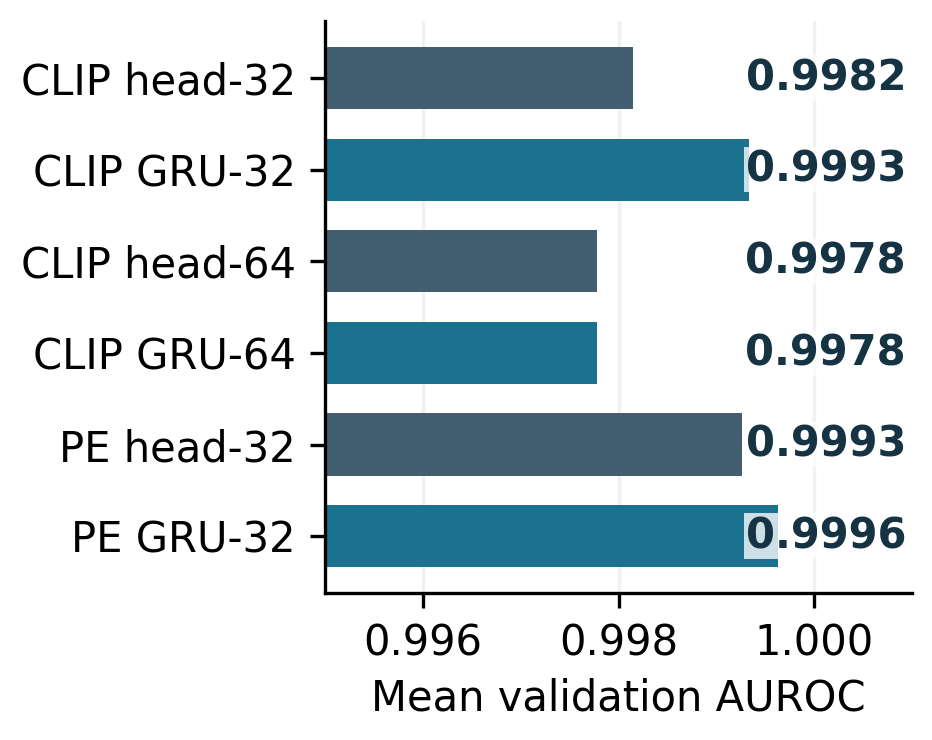
\includegraphics[width=0.98\columnwidth]{figures/fig03_validation_auroc.png}
\caption{Mean FaceForensics++ validation AUROC for released heads and five-seed GRU runs. The horizontal scale is zoomed to display small differences.}
\label{fig:3}
\end{figure}
\subsection{Held-out FaceForensics++ performance}
The final in-domain test contains 100 videos from 25 disjoint source groups. Fig. 4 compares probabilities averaged over the five seeds of each GRU configuration. CLIP-GRU-32 achieved 1.0000 AUROC after averaging seed probabilities, compared with 0.9972 for the released CLIP head. PE-GRU-32 attained 0.9992, and the GRU-pair ensemble attained 0.9996. These probabilities averaged across seeds are not the same statistic as mean metrics across separate runs \cite{capstone2026}.

\begin{figure}[!htbp]
\centering
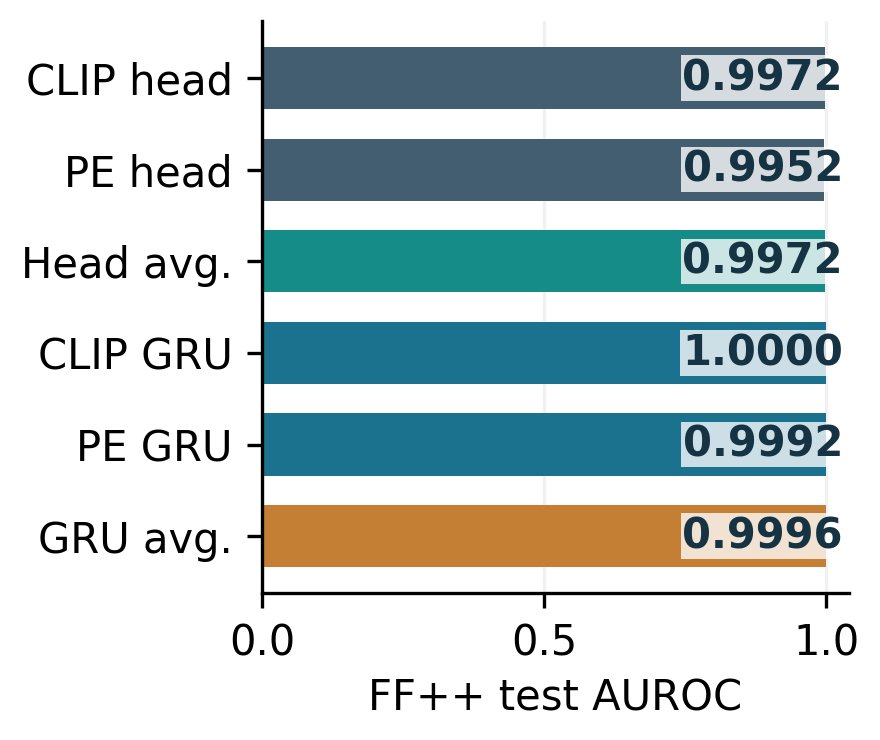
\includegraphics[width=0.98\columnwidth]{figures/fig04_ffpp_auroc.png}
\caption{FaceForensics++ c23 held-out AUROC for the six video-scoring configurations; results are based on the same 100 videos.}
\label{fig:4}
\end{figure}
\begin{figure}[!htbp]
\centering
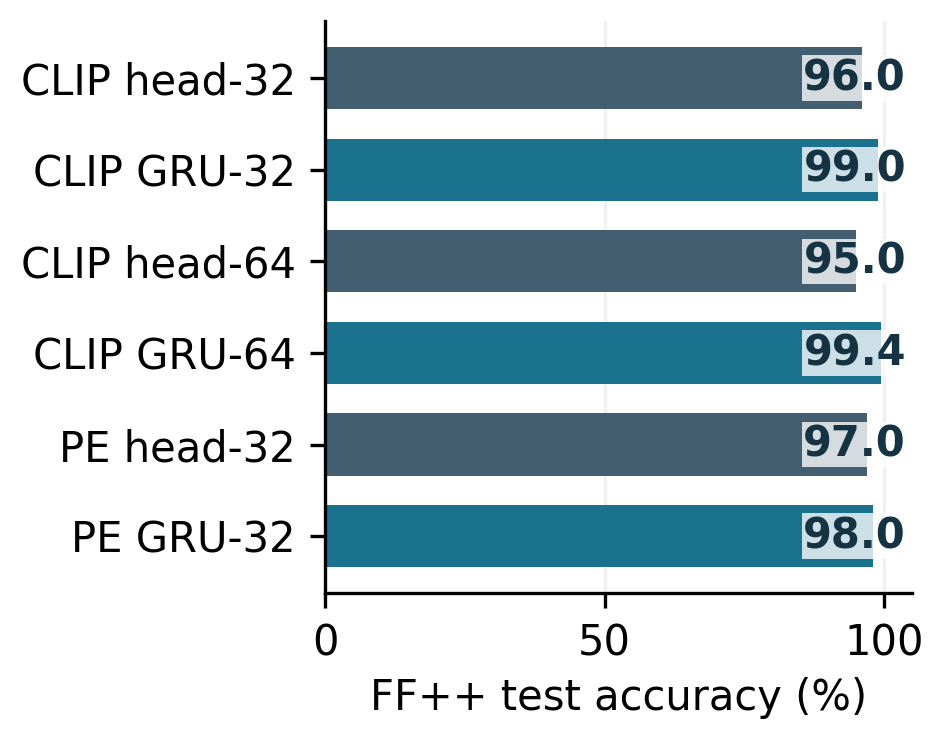
\includegraphics[width=0.98\columnwidth]{figures/fig05_ffpp_accuracy.png}
\caption{Mean held-out FaceForensics++ accuracy by backbone and frame setting. GRU figures are five-seed means; head results use released checkpoints.}
\label{fig:5}
\end{figure}
A separate per-seed analysis found CLIP-GRU-32 test AUROC 0.999680 ± 0.000335 and mean accuracy 99.0\%, compared with GenD-CLIP-32 AUROC 0.997200 and accuracy 96.0\%. The corresponding GRU-64 five-seed mean was 0.999840 AUROC with 99.4\% accuracy, but that secondary test result did not change the validation-based 32-frame selection. The original pilot had only four test videos and is not used as the main evidence. Fig. 5 reports the corresponding accuracy results \cite{capstone2026}.

\subsection{External Celeb-DF v2 generalization}
The official Celeb-DF v2 subset contains 518 videos, including 340 manipulated examples. Fig. 6 shows a substantive reversal of the in-domain ranking. The released-head ensemble reached 0.971216 AUROC; the CLIP- and PE-based GRUs reached 0.946299 and 0.943837 respectively, while averaging both GRUs improved them to 0.964045. These figures supersede the October presentation’s statement that cross-dataset GRU testing had not yet been completed \cite{li2020}, \cite{capstone2026}.

\begin{figure}[!htbp]
\centering
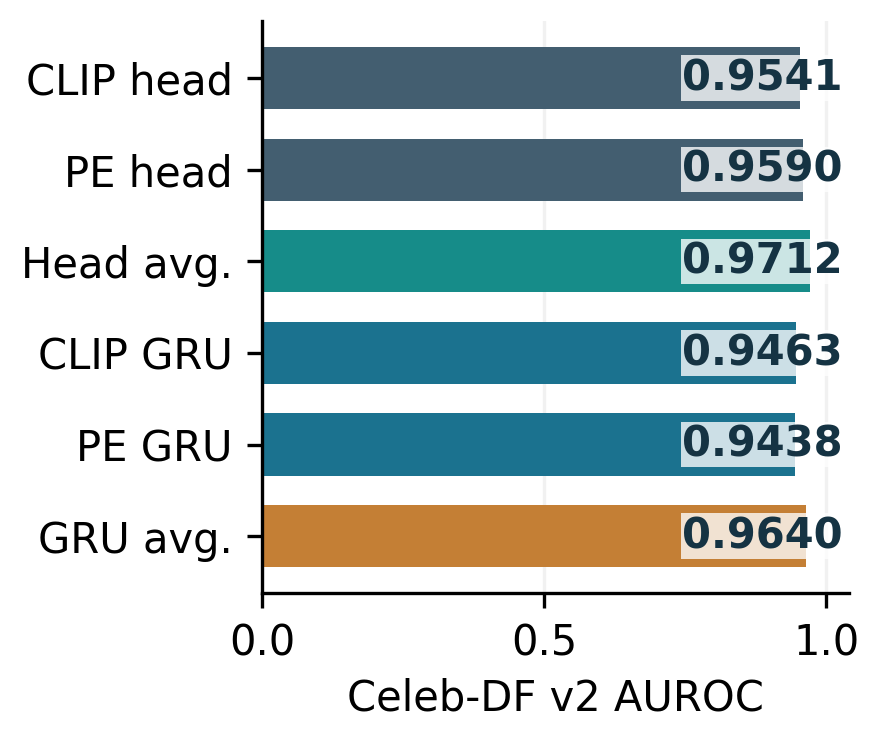
\includegraphics[width=0.98\columnwidth]{figures/fig06_celebdf_auroc.png}
\caption{Celeb-DF v2 external AUROC. The released-head CLIP+PE ensemble ranks above both individual GRUs and their ensemble.}
\label{fig:6}
\end{figure}
\subsection{Precision, errors, and constrained false alarms}
Fig. 7 reports AP. The released-head ensemble obtained 0.98146, compared with 0.97562 for the combined GRUs. This supports the AUROC ranking while measuring the precision-recall relationship. Fig. 8 shows that the released-head ensemble also attained a lower EER (9.20\%) than either GRU variant averaged together (10.78\%) \cite{capstone2026}.

\begin{figure}[!htbp]
\centering
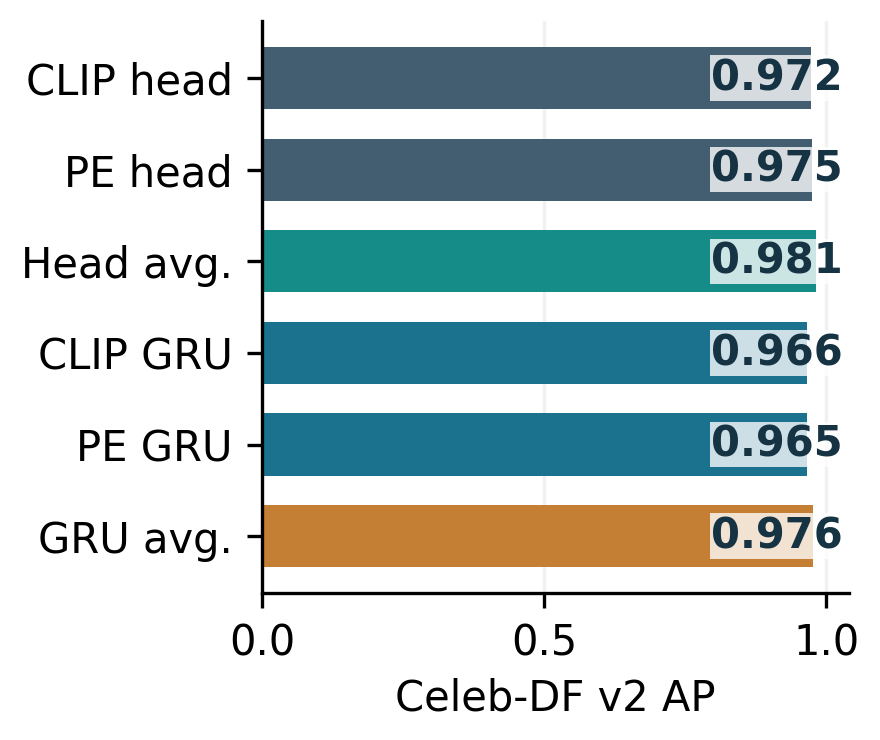
\includegraphics[width=0.98\columnwidth]{figures/fig07_celebdf_ap.png}
\caption{Average precision on Celeb-DF v2. Higher values indicate stronger precision-recall performance.}
\label{fig:7}
\end{figure}
\begin{figure}[!htbp]
\centering
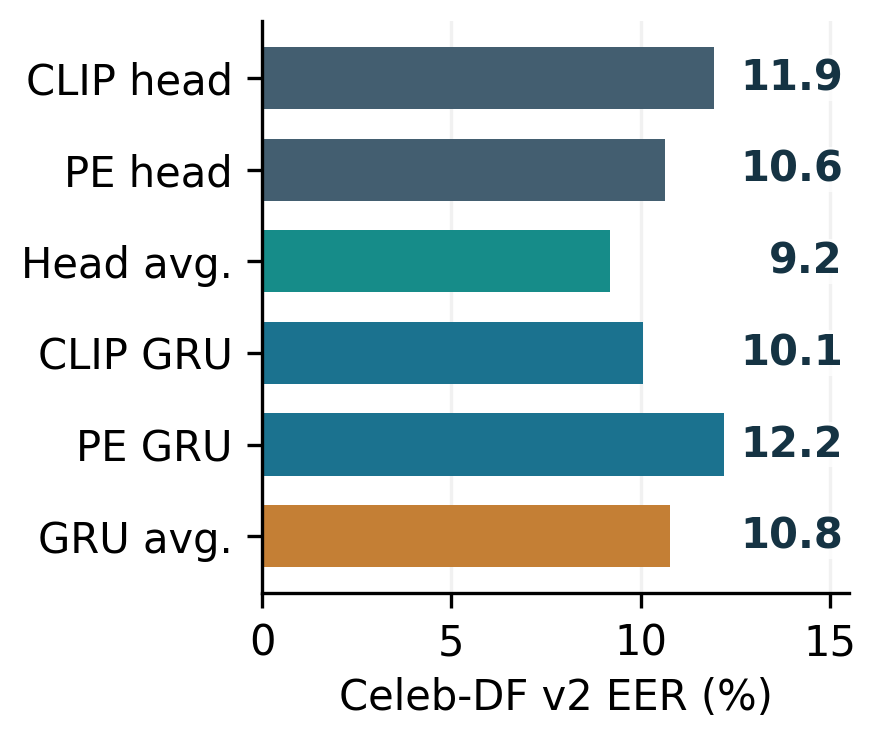
\includegraphics[width=0.98\columnwidth]{figures/fig08_celebdf_eer.png}
\caption{Equal-error rate on Celeb-DF v2. Lower is better; the two-head score ensemble reached 9.20\%.}
\label{fig:8}
\end{figure}
At a stringent 1\% false-positive rate, the released-head ensemble detected 56.2\% of manipulated videos, compared with 28.2\% for the GRU ensemble. As shown in Fig. 9, PE-GRU alone reached 33.8\% and CLIP-GRU 17.9\%. These threshold-dependent figures demonstrate why a high AUROC is insufficient to specify a deployment threshold. The threshold must be determined on separate validation data, not adjusted using the external test \cite{capstone2026}.

\begin{figure}[!htbp]
\centering
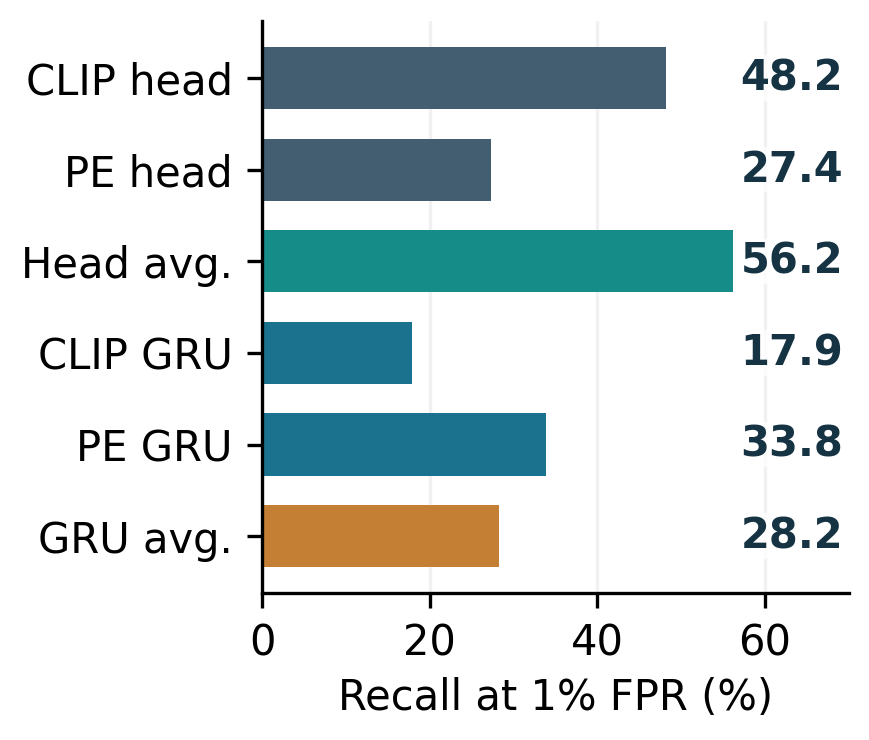
\includegraphics[width=0.98\columnwidth]{figures/fig09_celebdf_recall1.png}
\caption{Recall of manipulated Celeb-DF v2 videos at a 1\% false-positive rate. Larger values are better.}
\label{fig:9}
\end{figure}
At the more permissive 5\% false-positive operating point, the released-head ensemble reached 84.1\% recall, the GRU ensemble 82.4\%, CLIP-GRU 80.6\%, and PE-GRU 66.5\%. Fig. 10 contrasts these figures with the corresponding single-head results. Neither the 1\% nor the 5\% point is a deployment guarantee; both are observations on the external test labels \cite{capstone2026}.

\begin{figure}[!htbp]
\centering
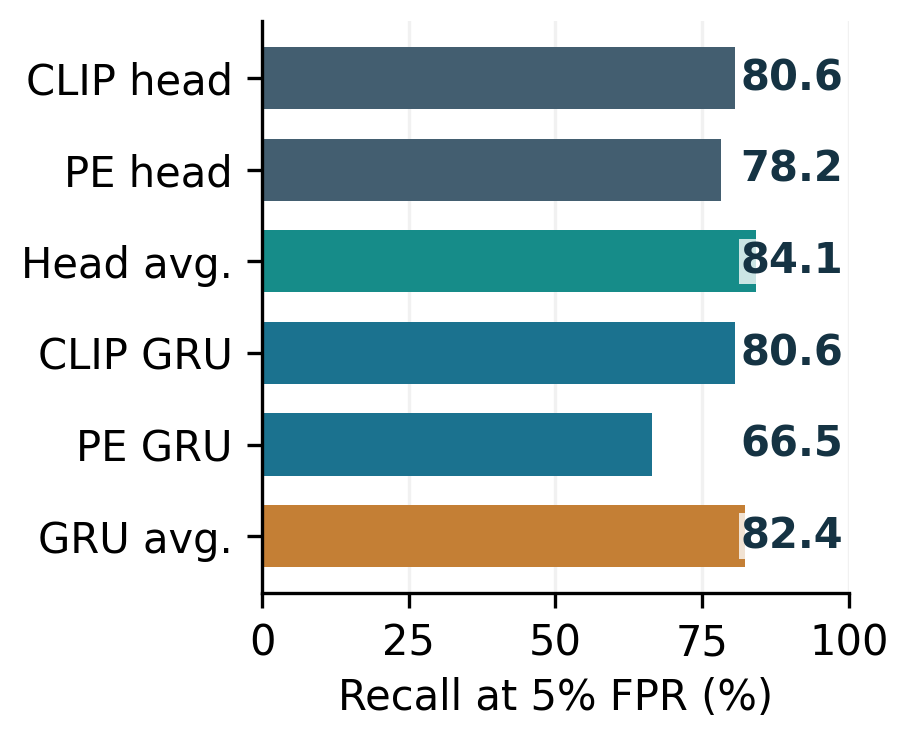
\includegraphics[width=0.98\columnwidth]{figures/fig10_celebdf_recall5.png}
\caption{Recall of Celeb-DF v2 manipulations at a 5\% false-positive rate for the six final detector configurations.}
\label{fig:10}
\end{figure}
\subsection{Seed variation and interpretation}
The five CLIP-GRU-32 seeds were not identical on held-out FaceForensics++ examples. The saved per-seed report records AUROCs of 0.9996, 1.0000, 0.9996, 0.9992, and 1.0000, while their accuracies range from 97\% to 100\%. The released 32-frame CLIP head made four errors on that split. Two GRU seeds corrected all four, but another introduced a new error. These cases show why the per-seed mean and the five-seed probability ensemble should be shown separately rather than selected retrospectively using the test set \cite{capstone2026}.

\subsection{Comparison uncertainty and validity}
Paired 2,000-resample bootstrap comparisons on Celeb-DF v2 found an AUROC gain for the released-head ensemble over CLIP of +0.01715 (95\% interval +0.00654 to +0.02948) and over PE of +0.01224 (+0.00537 to +0.02029). The GRU ensemble exceeded CLIP-GRU by +0.01775 (+0.00651 to +0.03027), but was below the released-head ensemble by 0.00717 (difference interval -0.01546 to -0.00008). In contrast, in-domain gains were near the ceiling and their bootstrap difference intervals reached zero \cite{capstone2026}.

The analysis shows two different achievements rather than a universal winner. Temporal models can learn accurate rankings of held-out examples from a familiar source distribution. Cross-dataset performance favors the simpler averaging of two separately released GenD classifiers. The results do not identify which artifact causes the GRUs to transfer less effectively; that question requires further controlled experiments.

\subsection{Training behavior and failure patterns}
The saved training logs show that a very small training loss does not guarantee better external transfer. At epoch 20, the mean CLIP-GRU-32 training BCE across five seeds had fallen to approximately 0.000016, while mean validation BCE was 0.102911. For PE-GRU-32, the corresponding values were 0.000063 and 0.081715. These are epoch-20 values rather than the selected-checkpoint losses. Their contrast illustrates why best-validation checkpointing and the independent external test remain essential \cite{capstone2026}.

The error audit further shows that model variance does not disappear merely because a test-set average is high. For the CLIP 32-frame baseline, three false positives and one false negative produced 96\% accuracy. At the same fixed threshold, independently trained GRU-32 seeds classified between 97 and 100 of the 100 videos correctly. The seed-probability ensemble achieved the highest in-domain AUROC, but that ranking was computed after averaging predictions, not by choosing the seed with the best held-out score \cite{capstone2026}.

The external comparison is more discriminating because the models are farther from the AUROC ceiling. The published-head ensemble improved the ranking of manipulated and genuine videos without new training, while both GRUs transferred less successfully. This observation supports the limited claim that complementary pretrained head scores are preferable for the particular Celeb-DF v2 evaluation. Whether temporal learning can recover the gap using diverse training manipulations, different frame-sampling rules, or calibrated outputs remains an open empirical question \cite{yermakov2026}, \cite{li2020}, \cite{capstone2026}.

\FloatBarrier
\clearpage
\section{DISCUSSION}
The research question concerned whether chronological GenD features improve video-level deepfake detection and whether combining complementary encoders offers a more dependable alternative. The in-domain FaceForensics++ comparison supports the first hypothesis in a narrow setting: CLIP-GRU-32 improved mean accuracy from 96.0\% to 99.0\%, and the averaged five-seed CLIP-GRU predictions perfectly ranked the small test set. Those results came from 100 videos whose source groups had not been used during GRU training. They still belong to the same compression condition and manipulation family as the training data \cite{rossler2019}, \cite{capstone2026}.

The external Celeb-DF v2 results change the interpretation. CLIP-GRU and PE-GRU reached 0.9463 and 0.9438 AUROC, both below the 0.9712 released-head ensemble. Combining the GRUs improved each component but did not restore the stronger external ranking of the released heads. One plausible explanation is that the GRUs learned temporal patterns useful for FaceForensics++ Deepfakes but less stable under a different manipulation process. We did not isolate generator features, so this remains a hypothesis rather than an experimentally verified cause \cite{li2020}, \cite{capstone2026}.

Model diversity is more consistently valuable on the external benchmark. The released-head ensemble improved AUROC relative to either head; paired bootstrap differences were positive. However, statistical evidence on one external dataset does not establish universal reliability. The same scores yield different recall at fixed false-positive rates, and mean-rank scores are not calibrated probabilities. A deployed detector would require a separate calibration set and a clear cost model for false alarms and missed manipulation \cite{capstone2026}.

The comparison also illustrates why different summary statistics should not be collapsed into one headline number. An AUROC of 1.0000 after averaging five CLIP-GRU model probabilities indicates perfect ranking on the tested 100 videos, not that every independent seed classified every sample correctly. Similarly, a favorable average BCE from an in-domain experiment does not prove calibrated probabilities on the external test. The independent-seed and ensemble metrics answer different reproducibility questions, and preserving their definitions prevents an inflated impression of model consistency \cite{capstone2026}.

There is a practical cost to the strongest external method. The released CLIP and PE heads must both evaluate face crops, increasing encoder compute and memory requirements relative to a single released head. Conversely, the GRUs are lightweight after feature extraction but cannot avoid obtaining CLIP or PE representations in the first place. A runtime comparison on the same video lengths, device, and preprocessing batch size is therefore needed before making a deployment recommendation on throughput. The team has developed a functioning local frontend, but the current sources do not provide a complete controlled cost benchmark for every final configuration \cite{capstone2026}.

Several limitations qualify the findings. The in-domain test is small and near the AUROC ceiling; bootstrap resampling of related videos may understate source dependence. The training set includes one selected FaceForensics++ manipulation type and compression profile, not the full space of deepfakes. Thirteen Celeb-DF videos needed repeated face crops, and the consequences of different crop distributions were not measured. The PE and CLIP encoders each add substantial computation, while the local frontend is a demonstration rather than a validated forensic product. Restricted FaceForensics++ video files must stay outside the public report package and repository \cite{rossler2019}, \cite{capstone2026}.

If the project continued for six months, the first phase would expand training to additional FaceForensics++ manipulations and audit per-source error patterns. A second phase would run strict cross-dataset evaluation on multiple untouched benchmarks, including crop-failure sensitivity and subgroup analyses with adequate sample sizes. A third phase would compare calibrated head ensembles, temporal models, and a jointly learned dual-backbone temporal architecture under a shared compute budget. The final phase would measure runtime, memory consumption, confidence stability, and robustness to video degradation. These are proposed studies, not completed results.

\FloatBarrier
\clearpage
\section{CONCLUSION}
This capstone evaluated two extensions to GenD video classification: chronological GRUs trained on frozen CLIP and PE features, and probability-level fusion of independently released classifiers. A source-group-separated FaceForensics++ experiment showed strong in-domain temporal performance, including 0.999680 mean per-seed AUROC for CLIP-GRU-32 and 1.0000 AUROC for its averaged five-seed predictions. External evaluation on 518 Celeb-DF v2 videos did not establish a generalization advantage for those GRUs. Instead, the released-head CLIP+PE ensemble achieved the strongest external AUROC of 0.9712 and the best recall at a 1\% false-positive rate among the six final configurations. The practical result is a reproducible comparison that favors simple complementary score fusion for the tested external distribution while retaining the temporal model as a useful, but distribution-sensitive, research extension.

\FloatBarrier
\clearpage
\appendices
\section{LaTeX Source Repository}
\begin{figure}[H]
\centering
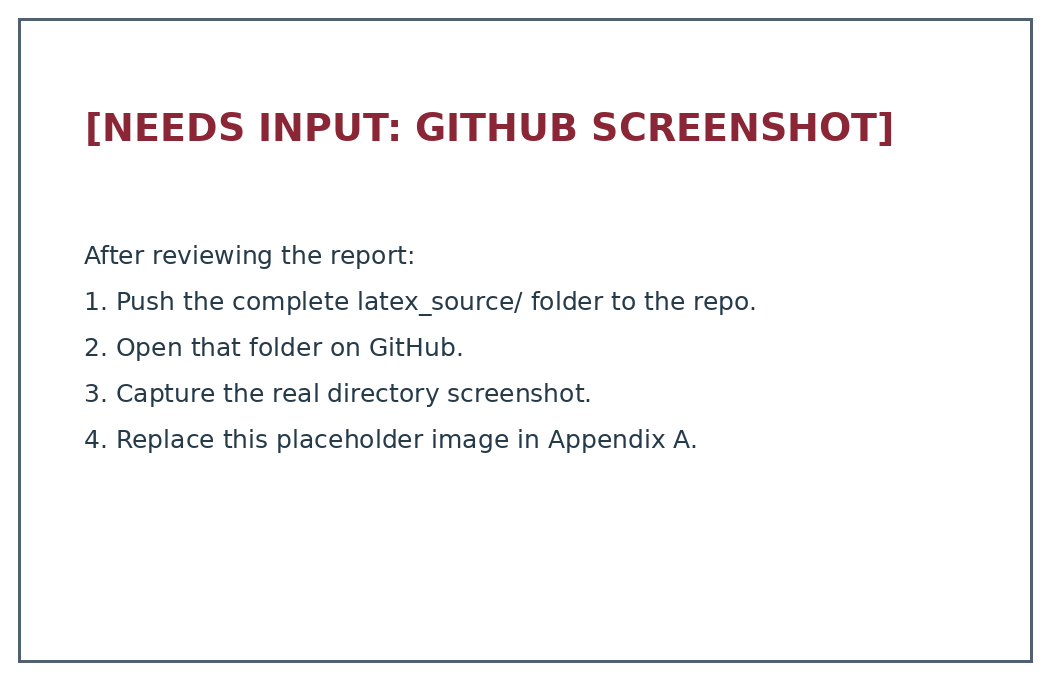
\includegraphics[width=0.99\columnwidth]{figures/fig11_APPENDIX_PLACEHOLDER.png}
\caption{[NEEDS INPUT: replace with a genuine GitHub screenshot of the uploaded latex\_source directory.]}
\end{figure}
\clearpage
\bibliographystyle{IEEEtran}
\bibliography{references}
\end{document}
